\documentclass[a4paper,12pt]{article} % добавить leqno в [] для нумерации слева
\usepackage[a4paper,top=1.3cm,bottom=2cm,left=1.5cm,right=1.5cm,marginparwidth=0.75cm]{geometry}
%%% Работа с русским языком
\usepackage{cmap}					% поиск в PDF
\usepackage{mathtext} 				% русские буквы в фомулах
\usepackage[T2A]{fontenc}			% кодировка
\usepackage[utf8]{inputenc}			% кодировка исходного текста
\usepackage[english,russian]{babel}	% локализация и переносы
\usepackage{multirow}

\usepackage{graphicx}

\usepackage{wrapfig}
\usepackage{tabularx}

\usepackage{hyperref}
\usepackage[rgb]{xcolor}
\hypersetup{
colorlinks=true,urlcolor=blue
}

%%% Дополнительная работа с математикой
\usepackage{amsmath,amsfonts,amssymb,amsthm,mathtools} % AMS
\usepackage{icomma} % "Умная" запятая: $0,2$ --- число, $0, 2$ --- перечисление

%% Номера формул
\mathtoolsset{showonlyrefs=true} % Показывать номера только у тех формул, на которые есть \eqref{} в тексте.

%% Шрифты
\usepackage{euscript}	 % Шрифт Евклид
\usepackage{mathrsfs} % Красивый матшрифт

%% Свои команды
\DeclareMathOperator{\sgn}{\mathop{sgn}}

%% Перенос знаков в формулах (по Львовскому)
\newcommand*{\hm}[1]{#1\nobreak\discretionary{}
{\hbox{$\mathsurround=0pt #1$}}{}}

%% Графики
\usepackage{tikz}
\usepackage{pgfplots}
\pgfplotsset{compat=1.9}

\date{\today}

\begin{document}

\begin{titlepage}
	\begin{center}
		{\large МОСКОВСКИЙ ФИЗИКО-ТЕХНИЧЕСКИЙ ИНСТИТУТ (НАЦИОНАЛЬНЫЙ ИССЛЕДОВАТЕЛЬСКИЙ УНИВЕРСИТЕТ)}
	\end{center}
	\begin{center}
		{\large Физтех-школа аэрокосмических технологий}
	\end{center}
	
	
	\vspace{4.5cm}
	{\huge
		\begin{center}
			{\bf Отчёт о выполнении лабораторной работы 1.2.5}\\
			Исследование вынужденной регулярной прецессии гироскопа
		\end{center}
	}
	\vspace{1cm}
	\begin{center}
		{\large Соболевский Фёдор Александрович \\
			\vspace{0.2cm}
			Б03-109}
	\end{center}
	\vspace{8cm}
	\begin{center}
		Октябрь 2021
	\end{center}
\end{titlepage}

\section{Аннотация}

В данной работе исследован гироскоп в кардановом подвесе и его вынужденная регулярная прецессия. Установлена зависимость скорости вынужденной прецессии от величины момента сил, действующих на ось гироскопа. Разными способами определена угловая скорость вращения ротора гироскопа. Оценены погрешности измерения угловой скорости каждым из способов. Проверена применимость приближённой теории гироскопа к реальному прибору.

\section{Теоретические сведения}

Уравнения движения твёрдого тела можно записать в виде

\begin{equation}
    \frac{d\vec{P}}{dt} = \vec{F},
    \label{NewtonLaw}
\end{equation}

\begin{equation}
    \frac{d\vec{L}}{dt} = \vec{F}.
    \label{momentEquation}
\end{equation}

Если сила $ \vec{F} $ не зависит от угловой скорости вращения системы, а момент $ \vec{M} $ - от скорости поступательного движения, то уравнения \eqref{NewtonLaw} и \eqref{momentEquation} можно рассматривать отдельно друг от друга. В данной работе рассматривается задача о вращении твёрдого тела вокруг неподвижной оси, которой соответствует последнее из уравнений.

Момент импульса твёрдого тела в его главных осях $ x, y, z $ равен

\begin{equation}
    \vec{L} = \vec{i}I_x\omega_x + \vec{j}I_y\omega_y + \vec{k}I_z\omega_z,
    \label{axisMoments}
\end{equation}

где $ I_x, I_y, I_z $ - главные моменты инерции, $ \omega_x, \omega_y, \omega_z $ - компоненты вектора угловой скорости $ \vec{\omega} $. Быстро вращающееся тело, для которого, например, $ I_z\omega_z \gg I_x\omega_x, I_y\omega_y $, принято называть гироскопом. Гироскоп называют уравновешенным, если его центр масс неподвижен. 

В силу \eqref{momentEquation} приращение момента импульса определяется интегралом

\begin{equation}
    \Delta \vec{L} = \int \vec{M} dt.
    \label{momentIncrement}
\end{equation}

\begin{figure}[h]
    \centering
    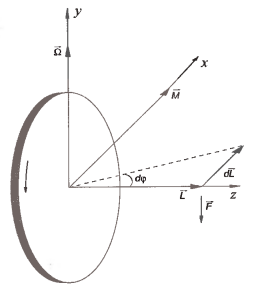
\includegraphics[width = 0.36\textwidth]{1.2.5 flywheel.PNG}
    \caption{Маховик}
    \label{fig:flywheel}
\end{figure}

Если момент внешних сил действует в течение короткого промежутка времени, из интеграла \eqref{momentIncrement} следует, что приращение $ \Delta \vec{L} $ момента импульса значительно меньше самого момента импульса: $ |\Delta \vec{L}| \ll |\vec{L}| $. С этим связана значительная устойчивость гироскопа после приведения его в быстрое вращение.

Выясним, какие силы надо приложить к гироскопу, чтобы изменить направление его оси. Рассмотрим для примера маховик, вращающийся вокруг оси $ z $, перпендикулярной к плоскости маховика (рис. \ref{fig:flywheel}). Будем считать, что $\omega_z = \omega_0, $ $\omega_x = \omega_y = 0 $. Пусть ось вращения повернулась в плоскости $ zx $ по направлению к оси $ x $ на бесконечно малый угол $ d\phi $. Такой поворот означает добавочное вращение маховика вокруг оси $ y $, так что $ d\varphi = \Omega dt $, где $ \Omega $ - угловая скорость такого вращения. Будем предполагать, что

\begin{equation}
    L_\Omega \ll L_{\omega_0}.
    \label{precessionReq}
\end{equation}

Это значит, что момент импульса маховика только повернётся в плоскости $ zx $ по направлению к оси $ x $ без изменения его величины. Отсюда

\begin{equation}
    |d\vec{L}| = L d\varphi = L\Omega dt. 
\end{equation}

Это изменение направлено вдоль оси $ x $, поэтому вектор d\vec{L} можно представить как векторное произведение вектора угловой скорости $ \vec{\Omega} $, направленного вдоль оси $ y $, на вектор собственного момента импульса маховика, направленного вдоль оси $ z $,

\begin{equation}
    d\vec{L} = \vec{\Omega} \times \vec{L} dt,
\end{equation}

то есть

\begin{equation}
    \frac{d\vec{L}}{dt} = \vec{\Omega} \times \vec{L}.
\end{equation}

В силу \eqref{momentEquation} имеем

\begin{equation}
    \vec{M} = \vec{\Omega} \times \vec{L}.
    \label{gyroEquation}
\end{equation}

Формула \eqref{gyroEquation} справедлива, если выполнено условие \eqref{precessionReq}. Из данного выражения видно, что для поворота оси вращения к оси $ x $ необходимо приложить силы, направленные вдоль оси $ y $, чтобы их момент был направлен к оси $ x $. $ \ddot{\text{и}}$

Под действием момента $ \vec{M} $ внешних сил ось гироскопа медленно вращается вокруг оси $ y $ с угловой скоростью $ \Omega $. Такое движение называется регулярной прецессией гироскопа. Для изучения регулярной прецессии уравновешенного гироскопа к его оси подвешивают дополнительные грузы, что создаёт момент сил тяжести, вызывающий прецессию. Её скорость в этом случае равна

\begin{equation}
    \Omega = \frac{mgl}{I_z\omega_0},
    \label{turnRate}
\end{equation}

где $ m $ - масса груза, $ l $ - расстояние от центра масс до точки крепления груза на оси гироскопа.

На практике в оси гироскопа возникает момент сил трения, что приводит к постепенному опусканию оси гироскопа во время прецессии. Оценить момент сил трения можно, по аналогии с моментом, вызывающим прецессию, умножив вертикальное изменение момента импульса на угловую скорость опускания оси вращения:

\begin{equation}
    M_\text{тр} = L \times \Omega_\text{тр} \approx L\Delta\varphi \times \frac{\Delta\varphi}{T} = I_z \omega_0 \frac{\Delta\varphi^2}{T},
    \label{frictionMoment}
\end{equation}

где $ \Delta\varphi $ - угол, на который опускается ось за период обращения.

\begin{figure}[h]
    \centering
    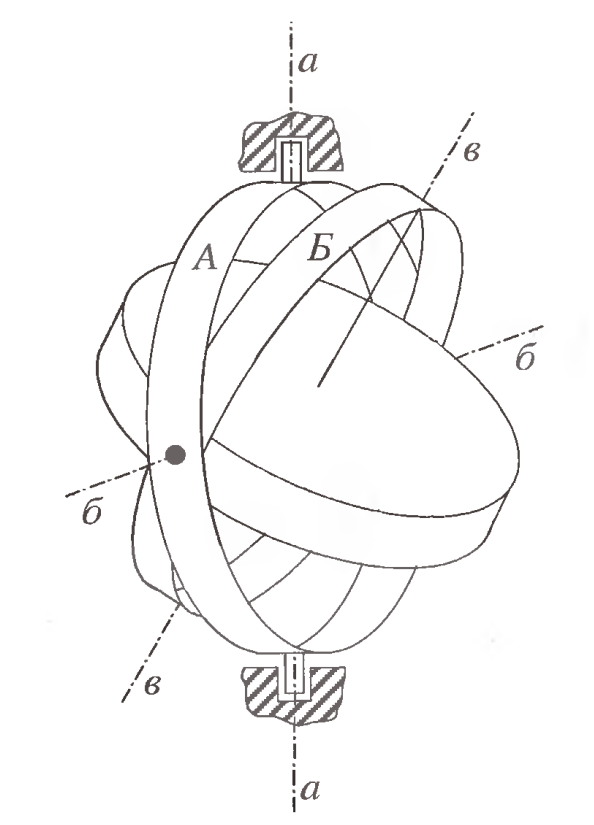
\includegraphics[width = 0.3\textwidth]{1.2.5 gyro.PNG}
    \caption{Гироскоп в кардановом подвесе}
    \label{fig:gyro}
\end{figure}

\begin{figure}[h]
    \centering
    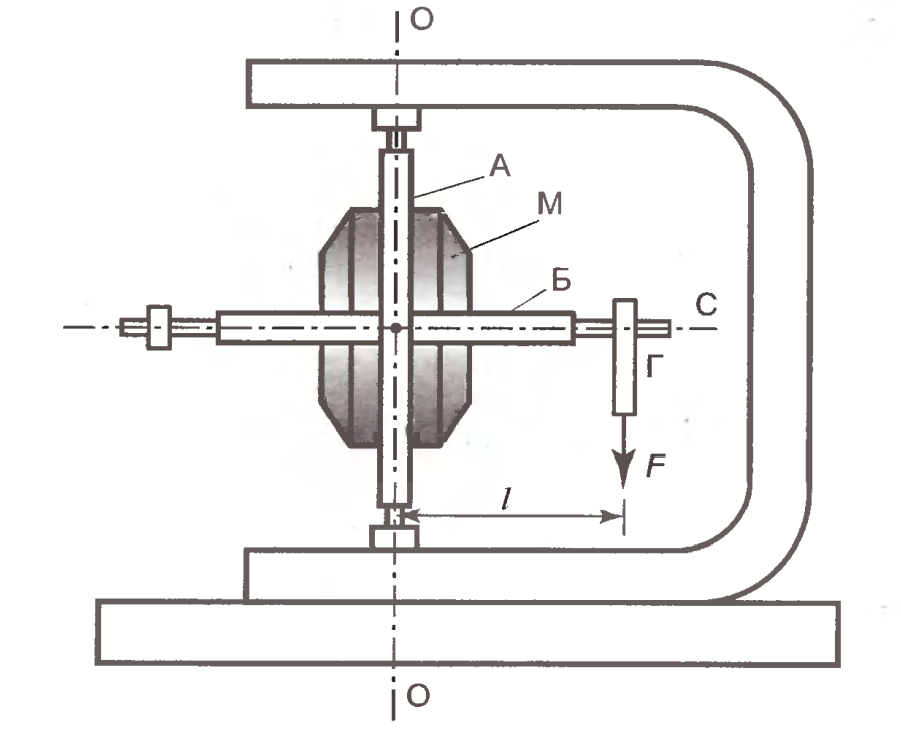
\includegraphics[width = 0.5\textwidth]{1.2.5 setup.PNG}
    \caption{Схема экспериментальной установки}
    \label{fig:setup}
\end{figure}

Уравновешенный гироскоп в кардановом подвесе, используемый в данной работе, показан на рисунке \ref{fig:gyro}. Центр масс гироскопа находится на пересечении трёх осей вращения карданова подвеса и при любом повороте колец сохраняет своё положение в пространстве.

Экспериментальная установка показана на рисунке \ref{fig:setup}. Ротором гироскопа является ротор высокооборотного электромотора M, питающегося током частотой 400 Гц. Кожух мотора (статор) скреплён с кольцом Б (рис. \ref{fig:gyro} и \ref{fig:setup}). Мотор с кольцом Б может вращаться в кольце А вокруг горизонтальной оси \textit{бб}. Кольцо А может вращаться вокруг горизонтальной оси \textit{аа}. Ротор электромотора представляет собой массивный стальной цилиндр с прожилками меди. Обозначенный на рис. \ref{fig:setup} буквой C рычаг направлен по оси симметрии ротора. Подвешивая на рычаг грузы Г, можно менять силу $ F $, момент которой определяется расстоянием l от точки подвеса до центра масс гироскопа (до горизонтальной оси кольца А), указанным на установке.

Измерение скорости прецессии гироскопа позволяет вычислить угловую скорость вращения его ротора по формуле \eqref{turnRate}. Момент инерции ротора относительно оси симметрии $ I_z $ можно измерить по периоду крутильных колебаниям точной копии ротора, подвешиваемой вдоль оси симметрии на жёсткой проволоке. Период крутильных колебаний $ T_0 $ зависит от момента инерции $ I_z $ и модуля кручения проволоки $ f $:

\begin{equation}
    T_0 = 2\pi\sqrt{\frac{I_z}{f}}
    \label{spinPeriod}
\end{equation}

Чтобы исключить из \eqref{spinPeriod} неизвестный модуль кручения, вместо ротора к той же проволоке следует подвесить цилиндр правильной формы, для которого можно легко вычислить момент инерции $ I_\text{ц} $. Для определения момента инерции ротора гироскопа из \eqref{spinPeriod} имеем

\begin{equation}
    I_z = I_\text{ц} \frac{T_0^2}{T_\text{ц}^2},
    \label{inertiaMoment}
\end{equation}

где $ T_\text{ц}^2 $ - период крутильный колебаний цилиндра. 

Скорость вращения ротора гироскопа можно определить также с помощью частотометра, подключенного к обмотке в статоре. Вращаясь, ротор создаёт в обмотке переменную ЭДС, частота которой равна частоте вращения ротора. Частоту этой ЭДС и измеряет частотометр с высокой точностью. 

\section{Оборудование и инструментальные погрешности}

\textbf{Оборудование:} гироскоп в кардановом подвесе, секундомер, набор грузов, отдельный ротор гироскопа, цилиндр известной массы, крутильный маятник, электронные весы, штангенциркуль, секундомер, частотометр.

\textbf{Инструментальные погрешности:}

\begin{itemize}
    \item \textbf{Штангенциркуль:} $ \Delta_l^\text{сист} = 0,1 $ мм;
    \item \textbf{Весы:} $ \Delta_m^\text{сист} = 0,1 $ г;
    \item \textbf{Секундомер:} $ \Delta_t^\text{сист} = 0,1 $ с;
    \item \textbf{Частотометр:} $ \Delta_\nu^\text{сист} = 0,01 $ Гц.
\end{itemize}

\section{Результаты измерений и обработка экспериментальных данных}

\subsection{Измерение скорости прецессии}

В данной работе скорость прецессии измерялась через период полного оборота гироскопа вокруг вертикальной оси при воздействии на него момента сил тяжести. Измерения проводились для пяти разных весов грузов. Для каждого веса $ N = 5 $ раз измерялось время $ T $ одного оборота, затем полученные значения усреднялись, и из среднего значения $ \overline{T} $ вычислялась угловая скорость прецессии

\begin{equation}
    \Omega = \frac{2\pi}{\overline{T}}.
\end{equation}

Погрешность вычисления среднего для данных величин

\begin{equation}
    \sigma_{\overline{T}}^\text{случ} = \frac{1}{N} \sqrt{\sum_{i = 1}^N (T_i - \overline{T})^2}\text{,      } \sigma_{\overline{T}} = \sqrt{(\sigma_{\overline{T}}^\text{случ})^2 + (\Delta_t^\text{сист})^2},  
\end{equation}

\begin{equation}
    \sigma_\Omega = 2\pi\frac{\sigma_{\overline{T}}}{\overline{T}}\Omega.
\end{equation}

За время измерений ось вращения гироскопа не отклонялась более чем на 5-6 градусов от горизонтального положения, что позволяет применять при расчётах соотношение \eqref{turnRate}. Плечо силы тяжести $ l = 122 $ мм.

Результаты измерений представлены в таблице \ref{tab:precessionData}. По результатам измерений видно, что, несмотря на меньший разброс значений периода обращения при больших скоростях прецессии, относительная погрешность её определения больше, чем при малых скоростях, из-за большего вклада систематической погрешности измерения.

\begin{table}[h]
    \centering
    \begin{tabular}{|c|c|c|c|c|c|c|c|c|c|c|} \hline
        № & $ m $, г & $ T_1 $, с & $ T_2 $, с & $ T_3 $, с & $ T_4 $, с & $ T_5 $, с & $ \overline{T} $, с & $ \sigma_{\overline{T}} $, с & $ \Omega $, $ 10^{-3} $ рад/с & $ \sigma_\Omega $, $ 10^{-3} $ рад/с \\ \hline
        1 & 56,7 & 181,6 & 180,9 & 180,1 & 181,1 & 180,6 & 180,92 & 0,26 & 34,7 & 0,3 \\ \hline
        2 & 92,7 & 110,8 & 110,0 & 111,3 & 110,8 & 111,8 & 110,80 & 0,22 & 56,7 & 0,7 \\ \hline
        3 & 140,8 & 73,6 & 72,4 & 72,2 & 72,8 & 73,3 & 72.86 & 0.26 & 86.2 & 1.9 \\ \hline
        4 & 219,5 & 47,6 & 47,1 & 47,6 & 47,2 & 47,3 & 47.36 & 0.14 & 132.7 & 2.3 \\ \hline
        5 & 341,8 & 30,8 & 30,9 & 30,5 & 30,6 & 30,6 & 30.68 & 0.12 & 205 & 5 \\ \hline
    \end{tabular}
    \caption{Результаты измерения скоростей прецессии и их погрешности}
    \label{tab:precessionData}
\end{table}

Зависимость скорости $ \Omega $ прецессии от момента $ M $ сил тяжести, где $ M = mgl $, представлена на рисунке \ref{fig:precessionSpeds}. Видно, что зависимость $ \Omega $ от $ M $ линейна, что говорит о применимости соотношения \eqref{turnRate}.

На графике также построена аппроксимирующая прямая $ \Omega = kM $, где $ k = \frac{1}{I_z \omega_0} $. Коэффициент $ k $ и погрешность его определения $ \sigma_k $ определены как

\begin{equation}
    k = \frac{\langle \Omega M \rangle}{\langle M^2 \rangle} = 0,503 \text{ с/кг},
\end{equation}

\begin{equation}
    \sigma_k = \sqrt{\frac{1}{N - 1}(\frac{\langle \Omega^2 \rangle}{\langle M^2 \rangle} - k^2)} \approx 0,002 \text{ с/кг}.
\end{equation}

\begin{figure}
\centering
\resizebox {0.7\textwidth} {!} {
\begin{tikzpicture}
\begin{axis}[minor tick num = 4, xlabel = {$ M $, $ 10^{-3} \cdot $ Н/м}, ylabel = {$ \Omega $, $10^{-3}\cdot \text{рад/с}$}, xmin = 0, xmax = 425, ymin = 0, ymax = 215 ]
\addplot[color=black, mark=x, only marks] coordinates{(67.9, 34.7)(110.9, 56.7)(168.5, 86.2)(262.7, 132.7)(409.1, 205)};
\addplot[color=blue] coordinates{(0, 0)(420, 211.46)};
\end{axis}
\end{tikzpicture}
}
\caption{Зависимость скорости прецессии от момента сил тяжести}
\label{fig:precessionSpeds}
\end{figure}

\subsection{Нахождение момента инерции ротора гироскопа}

Период крутильных колебаний ротора на проволоке составил $ T_0 = 4,11 с $. Для цилиндра период колебаний составил $ T_\text{ц} = 4,02 с $. Радиус цилиндра $ r = 30,6 $ мм, его масса $ m_\text{ц} = 1617,2 $ г. Отсюда его момент инерции

\begin{equation}
    I_\text{ц} = \frac{m_\text{ц}r^2}{2} = 7,571 \cdot 10^{-4} \text{ кг} \cdot \text{м}^2.
\end{equation}

Из соотношения \eqref{inertiaMoment} момент инерции ротора равен

\begin{equation}
    I_z = I_\text{ц}\frac{T_0^2}{T_\text{ц}^2} = 7,91 \cdot 10^{-4} \text{ кг} \cdot \text{м}^2.
\end{equation}

Погрешности вычисления моментов инерции

\begin{equation}
    \sigma_{I_\text{ц}} = \frac{1}{2} I_\text{ц} \sqrt{4(\frac{\Delta_l^\text{сист}}{r})^2 + (\frac{\Delta_m^\text{сист}}{m_\text{ц}})^2} \approx 0,025 \cdot 10^{-4}  \text{ кг} \cdot \text{м}^2,
\end{equation}

\begin{equation}
    \sigma_{I_z} = I_z \sqrt{4(\frac{\Delta_t^\text{сист}}{T_\text{ц}})^2 + 4(\frac{\Delta_t^\text{сист}}{T_\text{0}})^2 + (\frac{\sigma_{I_\text{ц}}}{I_\text{ц}})^2} \approx 0,04 \cdot 10^{-4}  \text{ кг} \cdot \text{м}^2.
\end{equation}

\subsection{Вычисление угловой скорости вращения ротора гироскопа}

Зная величины $ k = \frac{1}{I_z\omega_0} $, $ I_z $ и их погрешности, можно вычислить угловую скорость ротора $ \omega_0 $:

\begin{equation}
    \omega_0 = \frac{1}{kI_z} = 2512,2 \text{ рад/с}. 
\end{equation}

Погрешность вычисления $ \omega_0 $

\begin{equation}
    \sigma_{\omega_0} = \omega_0 \sqrt{(\frac{\sigma_k}{k})^2 + (\frac{\sigma_{I_z}}{I_z})^2} = 2,6 \text{ рад/с}. 
\end{equation}

\textbf{Итоговый результат:} \underline{$ \omega_0 = (2512,2 \pm 2,6) $ рад/с}.
\\
\\
Частота вращения ротора гироскопа также измерялась частотометром: $ \nu = (400,01 \pm 0,01) $ Гц, отсюда \underline{$ \omega = 2\pi\nu = (2513,34 \pm 0,06) $ рад/с}.

\subsection{Оценка момента сил трения}

По формуле \eqref{frictionMoment} можно оценить момент сил трения. Для массы грузов $ m = 56,7 $ г за период обращения $ T = 180,92 $ с ось вращения опустилась на угол $ \Delta\varphi \approx 11^\text{o} $. Отсюда

\begin{equation}
    M = I_z \omega_0 \frac{\Delta\varphi^2}{T} = 0,4 \cdot 10^{-3} \text{ Н/м}
\end{equation}

Отсюда видно, что момент сил трения в данном опыте на несколько порядков меньше момента сил тяжести, вызывающих прецессию. Более того, угол отклонения оси вращения гироскопа от горизонтали оставался мал во всех опытах, а скорость вращения ротора поддерживалась постоянной, поэтому можно не учитывать вклад сил трения в погрешность результата.

\section{Обсуждение результатов и вывод}

Отклонение полученного опытным путём значения угловой скорости вращения ротора отличается от значения, полученного с помощью прибора высокой точности ($ \varepsilon \ll 1\% $), меньше, чем на $ \sigma_{\omega_0} $. При этом относительная погрешность полученного результата также невелика: $ \varepsilon_\omega \approx 0,1 \% $. Это говорит о том, что данный метод применим для измерения угловой скорости вращения ротора гироскопа в случае, если нет возможности сделать это с помощью точного прибора. Все теоретические закономерности, рассмотренные в данной работе, выполнились в пределах точности эксперимента.

\end{document}
